\documentclass[../Bachelorarbeit.tex]{subfiles}
\begin{document}

\chapter{State of the Art}
\label{chap:state_of_the_art}

Für die Orientierung in dem weitläufigen Gebiet der mobilen Entwicklung ist es notwendig, einen Überblick über die verschiedenen Ansätze zu erhalten. 
Da für diese Ansätze meist mehrere Frameworks existieren wird anhand der Kriterien(siehe Abschnitt: \nameref{sec:kriterien_der_analyse}) das passende Framework ausgewählt und dessen charakteristischen Eigenschaften vorgestellt.
Im folgenden Abschnitt: \ref{sec:auswertung} - \nameref{sec:auswertung} werden die  projektbezogenen Vor- und Nachteile der vorgestellten Frameworks kommentiert und die Wahl des umzusetzenden Ansatzes getroffen.


\section{Kriterien der Analyse}
\label{sec:kriterien_der_analyse}

Sicherlich ist es während der Orientierungsphase sinnvoll, einen Blick über den Tellerrand zu wagen.
Durch die Definition bestimmter Rahmenbedingungen und einer damit verbundenen eingeschränkten Auswahl soll eine zielgerichtete Analyse ermöglicht werden.
Diese Rahmenbedingung orientieren sich zum größten Teil an den Projekt-Anforderungen(siehe Abschnitt \ref{sec:anforderungen} (\nameref{sec:anforderungen})) und sind in folgenden Punkten definiert:

\subsubsection*{Unterstützte Ziel-Plattformen}
\label{subsub:supported_plattforms}
Dieser Punkt wurde aus den Projekt-\nameref{sec:anforderungen} übernommen. 
Es müssen folgende Plattformen für das Projekt unterstützt werden.


\begin{itemize}
\item Android
\begin{itemize}
\item ab der Version 4.0 - Ice Cream Sandwich(\ac{API} 14) 
\end{itemize}
\item Windows Phone
\begin{itemize}
\item ab der Version 8.0 
\end{itemize}
\end{itemize}

\subsubsection*{Entwicklungsumgebung}
Unter Entwicklungsumgebung - ist in dieser Definition - die für die  Entwickeln des Projektes notwendig Infrastruktur gemeint. 

\begin{itemize}
\item Betriebssystem
\begin{itemize}
\item Die Entwicklung sowie die Wartung der Applikation muss mit einem 64Bit-Windows 8-System durchführbar sein.
\end{itemize}
\item \ac{IDE}
\begin{itemize}
\item Als \ac{IDE} sollte entweder Visual Studio oder eine Eclipse-basierende \ac{IDE} verwendet werden.
\end{itemize}
\item Programmiersprachen
\begin{itemize}
\item Als mögliche Programmiersprachen kommen C\#, Java oder Javascript in Frage
\end{itemize}
\end{itemize}


\subsubsection*{Kosten}
Da es sich bei der \ac{OJAD} um eine Gemeinnützige Institution mit strikt definierten Ressourcen handelt, sollten die Lizenzkosten für die Evaluierung möglichst gering gehalten werden. Kostenlose- sowie OpenSource-Frameworks werden priorisiert.   

\subsubsection*{Native Installation-Datei}
Es muss möglich sein, dass die Applikation als native Installations-Datei vorliegt. Dies ist für die einfache und zügige Verteilung des fertigen Produktes notwendig.
\newpage

\section{Hybrider Ansatz}
\label{subsec:hybrid_framework}

Der Hybride Ansatz verbindet die Entwicklung von Applikationen durch Webtechnologien mit den Vorteilen von nativen Frameworks. 
Die in Javascript, \ac{HTML}5 und \ac{CSS}3 geschriebene Web-Applikation werden mithilfe eines Hybriden-Frameworks in einen nativen Container verpackt.
Durch die "`Verpackung"' in den Container bieten sich im wesentlichen zwei Vorteile.
Ein Vorteil besteht darin, dass der Zugriff auf Hardware, Sensorik sowie Native Funktionen gegeben ist. 
Die Unterstützung der Zielplattform sowie der Funktionsumfang sind dabei von dem eingesetzten Framework abhängig.
Ein weiterer Vorteil besteht darin, dass die Applikation über die Plattform-Stores wie eine Native-App verteilt werden kann.



\subsection*{Adobe PhoneGap}
\label{subsec:phonegap}

\begin{comment}
Was ist Phonegap ?
\end{comment}


Durch den Einsatz von PhoneGap können Multiplattform-Lösungen auf der Basis von Hybriden-Apps realisiert werden. 
Nach der Entwicklung steht ein natives App zur Verfügung das - über die jeweiligen Shops der Zielplattform - wie eine Native-Applikation verteilt werden kann.
Adobe PhoneGap selbst basiert auf dem OpenSource Framework: Apache Cordova. \\
\\
Von den hier vorgestellten Frameworks unterstützt PhoneGap die meisten Mobilen-Plattformen. 
Im Gegensatz zu \nameref{subsec:xamarin} steht allerdings nicht die gesamte Funktionalität der Zielplattform zur Verfügung, sondern ausschließlich definierte Bereiche.

\subsubsection*{Merkmale}
\begin{itemize}
\item Entwicklungssprache: Javascript (für die Definition der Grafischen Oberfläche werden \ac{HTML} und \ac{CSS} eingesetzt.)
\item Kosten:  kostenlos 
\item \ac{IDE}: wird ohne \ac{IDE} verteilt
\item Unterstützte Plattformen: 
\begin{itemize}
\item \textbf{Android}
\item \textbf{Windows Phone}
\item Amazon Fire OS, BlackBerry 10, Firefox OS, iOS, Ubuntu, Windows 8, Tizen
\end{itemize}
\end{itemize}

\begin{comment}
Wie funktioniert Phonegap
\end{comment}

PhoneGap selbst bietet keine \ac{IDE} oder Grafische Oberfläche für die Entwicklung an. 
Sämtliche Operationen wie "`neue Projekte"' anlegen oder "`Projekte builden"' werden mithilfe der Kommandozeile ausgeführt. \\
Die Einrichtung der PhoneGap-Umgebung ist - von den hier vorgestellten Frameworks - die aufwendigste Lösung. 
Neben den benötigten \ac{SDK} der Zielplattformen muss der Pfad zu dem lokalen ANT\footnote{Apache ANT ist ein Programm das, durch eine zentrale Konfigurationsdatei gesteuert, Java-Quellcode kompiliert\parencite[Mehr Informationen finden Sie unter: ][]{ant_homepage}. }-Verzeichnis in dem Systempfad korrekt hinterlegt sein. 
Desweiteren muss vor der eigentlichen Installation NodeJS lokal verfügbar sein.
Mit dem Befehl \texttt{npm install -g phonegap} wird die Installation von Phonegap schlussendlich gestartet.\\

Nachdem das Projekt durch den \texttt{Create}-Befehl angelegt wurde, kann es zur 
weiteren Bearbeitung in die Eclipse-\ac{IDE} importiert werden.
Aus dem PhoneGap-Projekt wird durch den \texttt{Build}-Befehl eine Native-Installationsdatei erzeugt.
\\
\\
Ein Vorteil von PhoneGap besteht darin, dass der Code nicht an die unterschiedlichen Plattformen angepasst werden muss. 
Für die Verwendung von Nativen Funktionen, wird mittels Javascript auf die Bibliotheksfunktionen(PhoneGap Pluins) zugegriffen. 
Für diesen Zweck verwendet PhoneGap die Cordova-\ac{API} \parencites(vgl.)()[Seite 2, sowie]{phonegap_cookbook}[Abschnitt: PhoneGap oder Apache Cordova]{phonegapArtikel_heiseDev}\\
Diese wrapped die nativen Methoden und bietet einen Zugriff via Javascript an.(Siehe Abb.: \ref{fig:phonegap-architecture} (\nameref{fig:phonegap-architecture}))

\begin{figure}
\centering
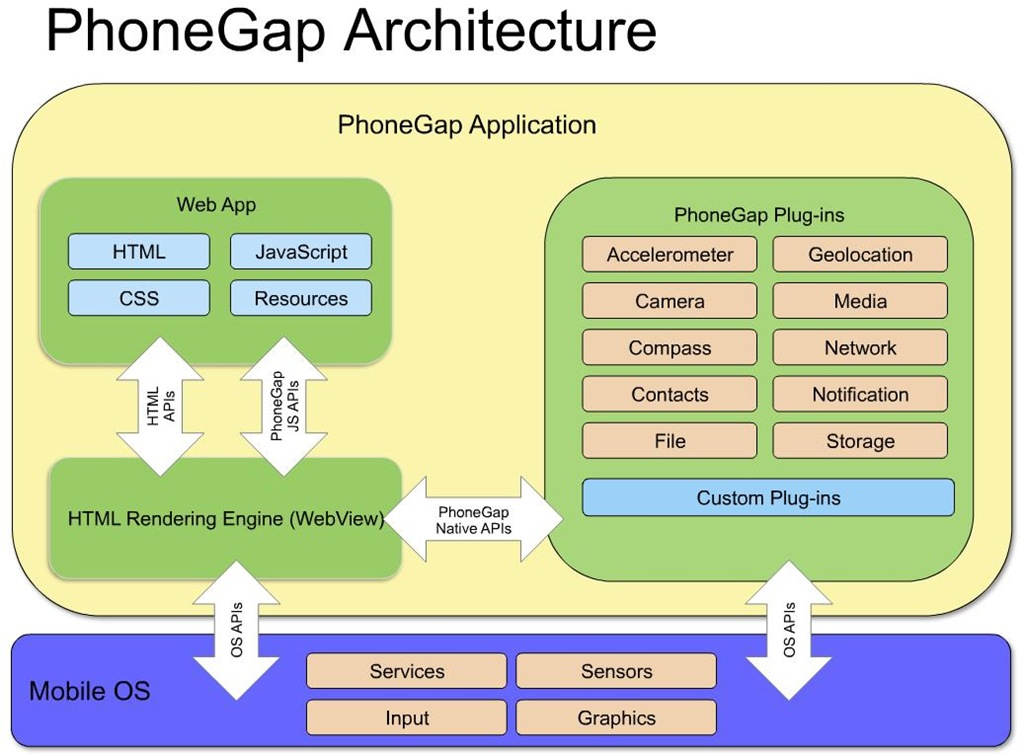
\includegraphics[width=0.8\linewidth]{./img/phonegap-architecture-by-ibm-29-july-2011-modules-instead-plug-ins}
\caption[PhoneGap Architektur]{PhoneGap Architektur \parencite[Quelle:][]{phonegap_Architektur}}
\label{fig:phonegap-architecture}
\end{figure}
\mbox{} \\
Für die Optimierung sowie Anpassung der grafischen Oberfläche können beliebige Mobile-Webframeworks wie \texttt{jQuery Mobile} oder \texttt{Sencha Touch} eingesetzt werden. 
Durch die Verwendung dieser Frameworks ist es möglich, dass die - mit PhoneGap entwickelte - App optisch einer Nativen-Applikation ähnelt.\\
\\
Neben dem verhältnismäßigen hohen Installationsaufwand\footnote{Im Vergleich zu den anderen Frameworks der State of the Art-Analyse.} besteht ein weiterer Nachteil darin, dass aktuell noch kein hochwertiger Debugger zur Verfügung steht.
Somit ist es aktuell noch nicht möglich, den Ablauf des Programmes auf allen unterstützten Endgeräten nachzuverfolgen. 
Adobe empfiehlt daher in Ihrem Wiki, das Projekt entweder in einem Desktop-Webbrowser
\footnote{Für das Debugging wird vom Hersteller empfohlen, einen Webbrowser zu verwenden, der auf dem \texttt{Webkit}-Engine basiert.} oder je nach Zielplattform, eine eigene Systemlösung zu verwenden\parencite[vgl.][]{phonegapWiki_debuging}.


 

\subsubsection*{Adobe PhoneGap Build}
\label{subsub:phonegap_build}

Seit September 2012 bietet Adobe den cloud-basierten Build-Service PhoneGap Build als Teil der Creative Cloud an\parencite[vgl.][]{phonegapBuild_launch}. 
PhoneGap Build steht zum einen kostenfrei sowie als Abonnement-Model zur Verfügung
\parencite[vgl.][ab Abschnitt: Choose your plan]{phonegapBuild_gebuehren}. 
Durch die Verwendung des Build-Services müssen die Zielplattformen nicht mehr lokal eingerichtet werden. 
Der Quelltext des Projektes wird entweder per Upload oder Link zu einem Github-Repository für den Build-Vorgang verfügbar gemacht.
Die erzeugten nativen Installationsdateien können anschließend heruntergeladen werden.
\newpage

\section{Interpretierter Ansatz}
Bei dem interpretierten Ansatz wird das Programm nicht in einer Maschinensprache sondern einer Interpretersprache codiert. 
Der Quellcode wird - zur Laufzeit - von dem Interpreter Zeile für Zeile ausgewertet und verarbeitet.
Innerhalb des Framework ist der benötigte Plattform-spezifische Code implementiert.
Dabei dient das verwendete Framework als Adapter zwischen dem Quellcode und der Zielplattform. 
Durch die ausgewerteten Anweisungen leitet der Interpreter die Ausführung der benötigten Operation des Frameworks ein.



\subsection*{Appcelerator Titanium}
\label{subsec:titanium}

Appcelerator Titanium ist ein auf dem interpretierten Ansatz basierendes Framework.
Wie bei \nameref{subsec:phonegap} wird als Entwicklungssprache Javascript eingesetzt. Im Gegensatz dazu muss bei nativen Apps kein \ac{HTML} verwendet werden. Allerdings ist es möglich, auch Mobile Web Applikationen mit Titanium zu erstellen(siehe Abb.: \ref{fig:titanium_studio_architecture} - \nameref{fig:titanium_studio_architecture}).


\subsubsection*{Merkmale}
\begin{itemize}
\item Entwicklungssprache: Javascript
\item Kosten:  kostenlos
\item \ac{IDE}: \nameref{subsub:titanium_studio}
\item Unterstützte Plattformen: 
\begin{itemize}
\item \textbf{Android}
\item \textbf{Windows Phone} derzeit noch nicht verfügbar, allerdings angekündigt \parencite[vgl.][]{titanium_wp8Support}
\item Tizen, BlackBerry
\end{itemize}
\end{itemize}
\newpage
\subsubsection*{Titanium \ac{SDK}}
\label{subsub:titanium_sdk}
Das Titanium-\ac{SDK}, welches in der nativen Sprache des Zielsystems entwickelt wurde, kann auf verschiedene Weisen erweitert werden. 
Neben Marketplace- sowie selbst entwickelten Modulen kann auch auf die Unterstützung von Cloud Services zugegriffen werden(siehe Abb.: \ref{fig:Titanium-Sdk} - \nameref{fig:Titanium-Sdk}). 
Diese Erweiterungen werden direkt über die \ac{IDE} \nameref{subsub:titanium_studio} in das Projekt eingebunden.
Es handelt sich nicht um einen Cross-Compile Vorgang wie er bei dem \nameref{subsec:xamarin}-Framework stattfindet. 
Stattdessen wurde der Javascript-Quellcode mit dem Titanium-\ac{SDK} zur Laufzeit durch den Interpreter der Endgerätes ausgeführt.

\begin{figure}
\centering
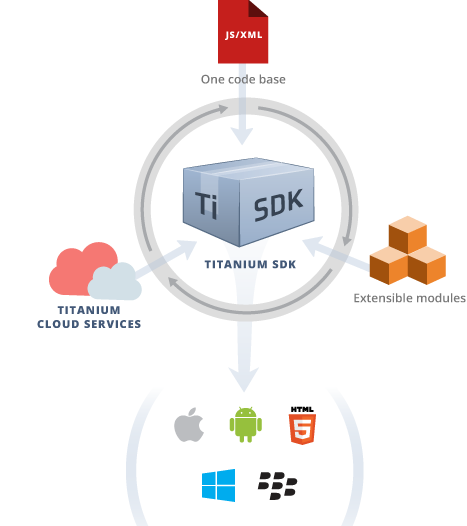
\includegraphics[width=0.6\linewidth]{./img/Titanium-Sdk}
\caption[Titanium \ac{SDK}]{Übersicht des Titanium-\ac{SDK}'s \parencite[Quelle:][]{titanium_sdk}}
\label{fig:Titanium-Sdk}
\end{figure}


\subsubsection*{Titanium Studio}
\label{subsub:titanium_studio}
Während der Entwicklung an einem Titanium-Projekt findet die Arbeit innerhalb der \ac{IDE} \nameref{subsub:titanium_studio} statt. 
\nameref{subsub:titanium_studio} basiert auf dem für Webentwicklung  spezialisierten \ac{IDE} Aptana Studio.
Als Abhängigkeit wird - wie bei dem \nameref{subsec:phonegap}-Framework - NodeJS benötigt, allerdings wird dies automatisch bei der Installation bezogen.\\
\\
Für den Bezug sowie den Start von \nameref{subsub:titanium_studio} ist ein kostenloser Appcelerator-Benutzeraccount notwendig.
Beim ersten Start führt ein Dialog durch die Einrichtung der gewünschten Plattformen.
Über den integrierten Marketplace können die im Abschnitt \ref{subsub:titanium_sdk} (\nameref{subsub:titanium_sdk}) erwähnten Module und Cloud Services bezogen werden. 
Die Integration der \ac{SDK}-Erweiterungen erfolgt in einer \ac{XML}-basierten Konfigurations-Datei des Projektes.
Ein Vorteil gegenüber \nameref{subsec:phonegap} besteht in dem von \nameref{subsub:titanium_studio} integrierten Debugger sowie der Unterstützung beim Einrichten der Zielplattformen. 

\begin{figure}
\centering
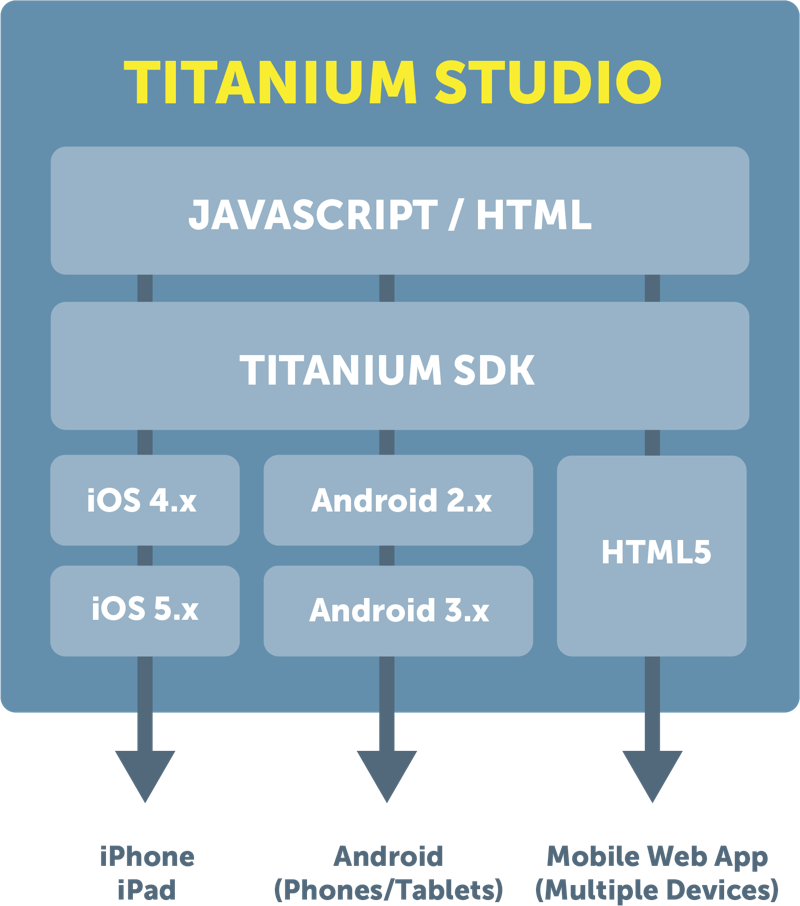
\includegraphics[width=0.8\linewidth]{./img/titanium_studio_architecture}
\caption[Titanium Architektur]{Titanium Architektur \parencite[Quelle:][]{titanium_architektur}}
\label{fig:titanium_studio_architecture}
\end{figure}


\newpage
\section{Übersetzender Ansatz}
Dieser Ansatz bezieht eine besondere Position. 
Im Gegensatz zu den vorhergegangenen Ansätzen wird der Quellcode nicht interpretiert sondern mit Hilfe von Plattform-Bibliotheken in kompilierten Maschinencode - für das jeweilige System - übersetzt.


\subsection*{Xamarin}
\label{subsec:xamarin}

Bei Xamarin handelt es sich um ein Framework, dass verschiedene Plattformen für die Entwicklung anbietet. 
Jede dieser Framework-Plattformen sind jeweils für ein Zielsystem wie beispielsweise Android ausgelegt. 
Durch den Einsatz von Xamarin kann mittels C\# auf die gesamte native \ac{API} zugegriffen werden \parencite[vgl. ][S. 10]{xamarin_whitepaper}.\\
\\
\subsubsection*{Merkmale}
\begin{itemize}
\item Entwicklungssprache: C\#
\item Kosten:  0 - 1.899 \$ 
\item \ac{IDE}: Xanmarine Studio (Eclipse) oder Visual Studio
\item Unterstützte Plattformen: 
\begin{itemize}
\item \textbf{Android}

\item Mac
\item \textbf{Windows Phone}
\end{itemize}
\end{itemize}

 
Durch die Möglichkeit, die gesamte \ac{API} des Zielsystemes zu verwenden(siehe Abb.: \ref{fig:XamarinPlattform} - \nameref{fig:Titanium-Sdk}), steht eine mit Xamarin erzeugte Applikation in den Punkten Aussehen sowie Funktionalität einer nativen Applikation in nichts nach. 
Dadurch ist es möglich, Teile des Quellcodes aus einer bestehenden C\#-Applikation plattformübergreifend zu verwenden. 
Allerdings müssen die systemspezifische Faktoren, wie beispielsweise die grafische Oberfläche, weiterhin für jede Zielplattform separat angepasst werden. 
Durch den Einsatz des - teilweise kostenpflichtigen - Component Store lässt sich das eigene Programm mit zusätzlichen Modulen und Bibliotheken wie beispielsweise Azure Mobile Services erweitern.\\
\\

Das Manko liegt in den verhältnismäßig hohen Lizenzkosten von Xamarin\footnote{Diese Aussage bezieht sich auf die Kosten von Xamarin im Vergleich zu den alternativen Frameworks.}. 
Je nach gewähltem Finanzierungsplan fallen zwischen 0 - 1.899 \$ pro Jahr, Entwickler und Plattform an \parencite[vgl.][] {xamarin_price}. 
Es ist zwar eine kostenlose Option verfügbar, allerdings ist diese stark limitiert.\footnote{Eine Restriktion besteht beispielsweise in der maximalen Größe des Quellcodes. \parencite[vgl.][]{xamarin_price_faq}} 
Somit muss mit jährlichen Kosten (pro EntwicklerInn) von mindestens 299\$, beziehungsweise 999\$ wenn die Visual Studio-Unterstützung gewünscht ist, gerechnet werden.

\begin{figure}
\centering
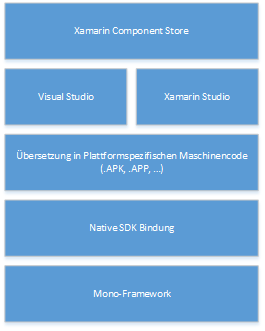
\includegraphics[width=0.6\linewidth]{./img/XamarinPlattform}
\caption{Xamarin Plattform \parencite[vgl.] [S. 8; Grafik wurde durch Autor angepasst]{xamarin_whitepaper}}
\label{fig:XamarinPlattform}
\end{figure}


\begin{comment}

\section*{Sonstige}

\begin{itemize} \color{red}
\item Kurze Vorstellung sonstiger Frameworks
\item z.B. Kivy, Sencha Touch
\end{itemize}
\end{comment}


\section{Nativer Ansatz}
\label{sec:nativer_ansatz}
Bei dem nativen Ansatz muss die Applikation für jede Plattform eigens implementiert werden.
Dafür wird jeweils das native \ac{SDK} verwendet.
Aufgrund der Spezifikation (siehe Abschnitt: \ref{subsub:supported_plattforms} - \nameref{subsub:supported_plattforms}) werden an dieser Stelle die beiden nativen \ac{SDK}'s vorgestellt.


\subsection*{Android Entwicklung}
Der Einstieg in die Android-Entwicklung ist denkbar einfach und ohne finanzielle Aufwände durchführbar. 
Für die Einrichtung der Entwicklungsumgebung ist es ausreichend, das Eclipse ADT bundle herunter zu laden und zu entpacken. 

\subsubsection*{Merkmale}
\begin{itemize}
\item Entwicklungssprache: Java 
\begin{itemize}
\item C/C++ (Android \ac{NDK})
\end{itemize}
\item Kosten:  kostenlos
\item \ac{IDE}: Eclipse \ac{ADT} oder Android Studio
\item Unterstützte Plattformen: 
\begin{itemize}
\item \textbf{Android}
\end{itemize}
\end{itemize}

Darin ist neben der - für Android angepassten - Eclipse-\ac{IDE} das \ac{SDK} sowie ein Abbild für den Android Emulator enthalten \parencite[siehe][]{android_getTheSdk}. 
Dies ist alles was für den Start notwendig ist. 
Der Einstieg in die Entwicklung soll durch das auf der Android-Entwicklerseite bereitgestellte Training erleichtert werden \parencite[siehe][]{android_training}. 
Anhand der Entwicklung einer Beispiel-Applikation werden die verschiedenen Elemente der Android-\ac{API} erläutert.
Für weiterführende Fragen befinden sich auf der Android-Entwicklerseite die  \ac{API}-Guides, sowie die - mit Beispielen dokumentierten - \ac{API}-Referenzen \parencites[vgl.][]{android_api_guides}[sowie][]{android_api_ref}.
EntwicklerInnen, die ihre Applikation über den Play-Store verteilen möchten, benötigen dafür eine Entwicklerlizenz.
Dies ist durch eine Registrierung über die "`Google Play-Developer Console"' möglich. Für die Registrierung fällt eine einmalige Gebühr in der Höhe von 25\$ an \parencite[vgl.][]{android_entwicklerregistrierung}

\subsection*{Windows Phone Entwicklung}
\label{sub:wp_entwicklung}

Der Download der "`Developer Tools"' im "`Windows Phone Dev Center"' ist der erste Schritt zur \nameref{sub:wp_entwicklung}.
In dem Software-Paket ist neben der \ac{IDE}: Visual Studio auch das benötigte Windows Phone \ac{SDK} enthalten.
Des weiteren kann von dem "`Windows Phone Dev Center"' der Windows Phone Emulator bezogen werden.


\subsubsection*{Merkmale}
\begin{itemize}
\item Entwicklungssprache: C\#
\item Kosten:  kostenlos
\item \ac{IDE}: Visual Studio
\item Unterstützte Plattformen: 
\begin{itemize}
\item \textbf{Windows Phone}
\end{itemize}
\end{itemize}




Um den Einstieg zu erleichtern bietet Microsoft auf der hauseigenen Bildungsplattform \ac{MVA} Lernvideos und Material für die \nameref{sub:wp_entwicklung} an.
Der Vorteil der \nameref{sub:wp_entwicklung} liegt in der Verfügbarkeit des \texttt{.NET}-Frameworks.
Dadurch haben die Entwickler Zugriff auf Techniken wie Databinding, \ac{XAML} und das \ac{MVVM}-Konzept, was die Entwicklung und Implementierung unterstützen soll.\\
\\
Für das Ausführen und Testen der Applikation werden zwei Optionen angeboten.
Zum einen kann das Programm, direkt aus Visual Studio, auf das Windows Phone 8-Gerät kopiert und im Debug-Modus gestartet werden. 
Für diesen Vorgang muss das Endgerät allerdings registriert sein. 
Um diese Registrierung durchführen zu können, benötigt der/die EntwicklerIn wiederum Zugriff auf einen aktiven "`developer account"', der mit jährlichen Kosten verbunden ist \parencite[vgl.][]{wp8_account-kosten}.
Zum anderen kann das Programm, ebenfalls im Debug-Modus, über Visual Studio auf dem Emulator ausgeführt werden. 
Für diese Option wird kein "`developer account"' benötigt.
Allerdings verfügt der Emulator über relativ hohe Systemanforderung.
Diese sind - unter anderen - Hyper-V, \ac{SLAT}, mindestens Windows 8 in der 64-Bit Pro-Edition und vier \ac{GB} \ac{RAM} \parencite[vgl.][]{wp8_emulator_requirement}.
 
\begin{comment}
Die Registrierung als  
Allerdings ist dafür die  nötig. 
Die wiederum mindestens  
Seit geraumer Zeit versucht Microsoft - im mobilen Markt - Fuß zu fassen und versucht dafür EntwicklerInnen von der Windows Phone-Plattform zu begeistern.
Aktuell ist das Angebot von Applikation im internen Phone Store - im Vergleich zu anderen Plattformen - aber noch übersichtlich \parencite[vgl.][]{store_vergleich}.
\end{comment}



\section{Auswertung}
\label{sec:auswertung}

Nach der Analyse der verschiedenen Frameworks soll an dieser Stelle die Auswahl des - im Projekt eingesetzten - Frameworks getroffen und begründet werden. 
Die Aufzählungen der Begründung findet in der selben Reihenfolge wie die Analyse statt und soll keine Reihung darstellen. 
Die Begründungen für diese Entscheidungen sind nicht im Allgemeinen (für jedes Projekt) gültig, sondern basieren - in erster Linie - auf den Projekt-\nameref{sec:anforderungen} des \ref{chap:einfuehrung}. Kapitels, sowie den - davon abgeleiteten und erweiterten - \nameref{sec:kriterien_der_analyse} des \ref{chap:state_of_the_art}. Kapitels. 

\subsection*{\nameref{subsec:phonegap}}
\nameref{subsec:phonegap} beeindruckt durch die schnelle und komfortable Entwicklung mittels Webtechnologien, sowie dem Vorteil, dass der Code nur einmal implementiert wird und nicht auf die verschiedenen Plattformen angepasst werden muss. Die geringeren Probleme mit der Einrichtung der Entwicklungsumgebung (Abhängigkeiten) können mit der Verwendung von \nameref{subsub:phonegap_build} umgangen werden.
\nameref{subsec:phonegap} ist in der engeren Auswahl und wird - bei zukünftigen Projekten -als Kandidat in Betracht gezogen. 

\subsection*{\nameref{subsec:titanium}}
Die Vorzüge der komfortablen \ac{IDE} mit dem inkludierten Debugger sowie die einfache Erweiterbarkeit des \nameref{subsub:titanium_sdk} zeichnen \nameref{subsec:titanium} aus. 
Leider scheidet es aufgrund des Punktes: \nameref{subsub:supported_plattforms} aus der Definition: \nameref{sec:kriterien_der_analyse} des \ref{chap:state_of_the_art}. Kapitels, aus. 
Es ist zwar die Unterstützung für Windows Phone 8 angemeldet \parencite[siehe: ][]{titanium_wp8Support}, allerdings ist diese - zum aktuellen Zeitpunkt - noch nicht verfügbar.

\subsection*{\nameref{subsec:xamarin}}
Der Hauptvorteil von \nameref{subsec:xamarin}liegt in der Wiederverwendbarkeit von existierenden C\#-Codes.
Dieser Vorteil kommt in dem aktuellen Projekt nicht zum Tragen, da kein bestehender Code existiert. 
Nichtsdestotrotz muss die Oberfläche für jede Applikation separat entwickelt werden.
Allerdings kann der plattformunabhängige Teil (Logik und Kommunikation) der Windows Phone Applikation im Android-Projekt wiederverwendet werden, wenn \nameref{subsec:xamarin} verwendet wird. 
Dennoch rechtfertigen die Vorteile von \nameref{subsec:xamarin} nicht die notwendige Investition\footnote{Diese Aussage betrifft die Meinung des Autors zu dem vorliegenden Projekt.} \parencite[siehe:][]{xamarin_price}. 


\subsection*{\nameref{sec:nativer_ansatz}}

Der native Ansatz bietet den Entwicklern die Freiheit, dass gesamte \ac{SDK} der Plattform zu nutzen. 
Neben den Vorteilen der nativen Oberflächen Gestaltung sowie der Performance entfallen Abhängigkeiten gegenüber Dritten (Frameworks).
Der Einsatz von nativen Oberflächen der jeweiligen Plattformen ist in diesem Projekt aufgrund der definierten \nameref{sub:ziele_der_gestaltung} (siehe Abschnitt: \ref{sub:ziele_der_gestaltung} - \nameref{sub:ziele_der_gestaltung}) notwendig.
An dieser Stelle ist anzumerken, dass die zuvor getroffene Aussage bezüglich der Performance nicht generell gültig ist. 
Durch Fehlentscheidungen in der Entwicklung sowie der Implementierung, kann die Performance einer nativen Applikation stark abfallen. \\
\\
Es ist möglich, dass der Einsatz von Abhängigkeiten (Frameworks) - in  gewissen Fällen - zu Problemen führen kann. 
Daher gilt es unter anderem zu beachten, inwiefern die Frameworks  gegenüber neuen Plattform-Updates kompatibel sind.
Diese Thematik spielt dann eine Rolle, wenn das Projekt in der Zukunft mit einem neuen Feature erweitert werden soll.\\ 
\\
Trotz des Nachteils, der fehlenden Codebasis für beide Ziel-Plattformen, fällt die Entscheidung auf Grund der erwähnten Vor- und Nachteile zu Gunsten des \textbf{nativen Ansatzes} aus\footnote{Ein weiterer Grund für die Entscheidung, ist der Wunsch einer nativen App von Seiten der \ac{OJAD}}.


\end{document}